%%%%%%%%%%%%%%%%%%%%%%%%%%%%%%%%%%%%%%%%%%%%%%%%%%%%%%%%%%%%%%%%%%%%%%%%%%%%%%%%%%%%%%%%%%%%%%%%%%%%%%%%%%%%%%%%%%%%%%%%%%%%%%%%%%%%%%%%%%%%%%%%%%%%%%%%%%%
% This is just an example/guide for you to refer to when submitting manuscripts to Frontiers, it is not mandatory to use Frontiers .cls files nor frontiers.tex  %
% This will only generate the Manuscript, the final article will be typeset by Frontiers after acceptance.   
%                                              %
%                                                                                                                                                         %
% When submitting your files, remember to upload this *tex file, the pdf generated with it, the *bib file (if bibliography is not within the *tex) and all the figures.
%%%%%%%%%%%%%%%%%%%%%%%%%%%%%%%%%%%%%%%%%%%%%%%%%%%%%%%%%%%%%%%%%%%%%%%%%%%%%%%%%%%%%%%%%%%%%%%%%%%%%%%%%%%%%%%%%%%%%%%%%%%%%%%%%%%%%%%%%%%%%%%%%%%%%%%%%%%

%%% Version 3.3 Generated 2016/11/10 %%%
%%% You will need to have the following packages installed: datetime, fmtcount, etoolbox, fcprefix, which are normally inlcuded in WinEdt. %%%
%%% In http://www.ctan.org/ you can find the packages and how to install them, if necessary. %%%
%%%  NB logo1.jpg is required in the path in order to correctly compile front page header %%%

\documentclass[utf8]{frontiersSCNS} % for Science, Engineering and Humanities and Social Sciences articles
%\documentclass[utf8]{frontiersHLTH} % for Health articles
%\documentclass[utf8]{frontiersFPHY} % for Physics and Applied Mathematics and Statistics articles

%\setcitestyle{square} % for Physics and Applied Mathematics and Statistics articles
\usepackage{url,hyperref,lineno,microtype,subcaption}
\usepackage[onehalfspacing]{setspace}
\usepackage{graphicx}
\usepackage{listings}
\usepackage{color}
\usepackage{lscape}
\usepackage[T1]{fontenc}
\usepackage{tikz}

\definecolor{mygreen}{rgb}{0,0.6,0}
\definecolor{mygray}{rgb}{0.5,0.5,0.5}
\definecolor{mymauve}{rgb}{0.58,0,0.82}

\lstset{ %
  backgroundcolor=\color{white},   % choose the background color; you must add \usepackage{color} or \usepackage{xcolor}; should come as last argument
  basicstyle=\footnotesize,        % the size of the fonts that are used for the code
  breakatwhitespace=false,         % sets if automatic breaks should only happen at whitespace
  breaklines=true,                 % sets automatic line breaking
  captionpos=b,                    % sets the caption-position to bottom
  commentstyle=\color{mygreen},    % comment style
  deletekeywords={...},            % if you want to delete keywords from the given language
  escapeinside={\%*}{*)},          % if you want to add LaTeX within your code
  extendedchars=true,              % lets you use non-ASCII characters; for 8-bits encodings only, does not work with UTF-8
  frame=single,	                   % adds a frame around the code
  keepspaces=true,                 % keeps spaces in text, useful for keeping indentation of code (possibly needs columns=flexible)
  keywordstyle=\color{blue},       % keyword style
  language=Octave,                 % the language of the code
  morekeywords={*,...},            % if you want to add more keywords to the set
  numbers=left,                    % where to put the line-numbers; possible values are (none, left, right)
  numbersep=5pt,                   % how far the line-numbers are from the code
  numberstyle=\tiny\color{mygray}, % the style that is used for the line-numbers
  rulecolor=\color{black},         % if not set, the frame-color may be changed on line-breaks within not-black text (e.g. comments (green here))
  showspaces=false,                % show spaces everywhere adding particular underscores; it overrides 'showstringspaces'
  showstringspaces=false,          % underline spaces within strings only
  showtabs=false,                  % show tabs within strings adding particular underscores
  stepnumber=2,                    % the step between two line-numbers. If it's 1, each line will be numbered
  stringstyle=\color{mymauve},     % string literal style
  tabsize=2,	                   % sets default tabsize to 2 spaces
  title=\lstname                   % show the filename of files included with \lstinputlisting; also try caption instead of title
}



% Leave a blank line between paragraphs instead of using \\


\def\keyFont{\fontsize{8}{11}\helveticabold }
\def\firstAuthorLast{Sample {et~al.}} %use et al only if is more than 1 author
\def\Authors{First Author\,$^{1,*}$, Co-Author\,$^{2}$ and Co-Author\,$^{1,2}$}
% Affiliations should be keyed to the author's name with superscript numbers and be listed as follows: Laboratory, Institute, Department, Organization, City, State abbreviation (USA, Canada, Australia), and Country (without detailed address information such as city zip codes or street names).
% If one of the authors has a change of address, list the new address below the correspondence details using a superscript symbol and use the same symbol to indicate the author in the author list.
\def\Address{$^{1}$Laboratory X, Institute X, Department X, Organization X, City X , State XX (only USA, Canada and Australia), Country X \\
$^{2}$Laboratory X, Institute X, Department X, Organization X, City X , State XX (only USA, Canada and Australia), Country X  }
% The Corresponding Author should be marked with an asterisk
% Provide the exact contact address (this time including street name and city zip code) and email of the corresponding author
\def\corrAuthor{Corresponding Author}

\def\corrEmail{email@uni.edu}




\begin{document}
\onecolumn
\firstpage{1}

\title[NWB Query Engine]{NWB Query Engine: Efficient way to query neurophysiological data stored in Neurodata Without Borders format} 

\author[\firstAuthorLast ]{\Authors} %This field will be automatically populated
\address{} %This field will be automatically populated
\correspondance{} %This field will be automatically populated

\extraAuth{}% If there are more than 1 corresponding author, comment this line and uncomment the next one.
%\extraAuth{corresponding Author2 \\ Laboratory X2, Institute X2, Department X2, Organization X2, Street X2, City X2 , State XX2 (only USA, Canada and Australia), Zip Code2, X2 Country X2, email2@uni2.edu}


\maketitle
  

\begin{abstract}

%%% Leave the Abstract empty if your article does not require one, please see the Summary Table for full details.
\section{}
For full guidelines regarding your manuscript please refer to \href{http://www.frontiersin.org/about/AuthorGuidelines}{Author Guidelines}.

As a primary goal, the abstract should render the general significance and conceptual advance of the work clearly accessible to a broad readership. References should not be cited in the abstract. Leave the Abstract empty if your article does not require one, please see \href{http://www.frontiersin.org/about/AuthorGuidelines#SummaryTable}{Summary Table} for details according to article type. 


\tiny
 \keyFont{ \section{Keywords:} keyword, keyword, keyword, keyword, keyword, keyword, keyword, keyword} %All article types: you may provide up to 8 keywords; at least 5 are mandatory.
\end{abstract}


\section{Introduction}

Data coming from neurophysiological experiments are heterogeneous and organized in various data formats. A data format is usually given by hardware and software equipment defined by the specific device vendor. This format cannot be easily changed or reused in different devices. Nowadays with increasing computational performance and disk storages capacity researchers are more and more motivated to preserve not only experimental results but also original data used for performing analysis. A new modern concept calls such data as "Big Data" defined as  three Vs. (1) Volume defining big data as data from variety of sources , (2) Velocity defining big data as data coming from sensors by unprecedented speed, and	(3) Variety saying that data are in all types of formats. Moreover, neurophysiological data go even more behind this concept. Their are multimodal and dynamic because single experiment can involve several signal acquisition modalities. With increasing number of experiments the problem of non-standarised datasets stored in non-standarised formats makes  difficult an effective management and sharing. Researchers point out that data are even more important then papers describing results observed from the data. It is because if results are described in scientific papers without an access to the original datasets their validation or refinement over time is practically impossible. As a solution several attempts to provide a standardized way of data storing have appeared. These approaches vary from free-form data storages based on a simple data model providing only basic data structure \citep{10.3389/fninf.2011.00016} to rigid data formats often based on fixed schema technologies implemented in relational databases (e. g. SciDB \citep{Brown:2010:OSL:1807167.1807271}) requiring strictly defined set of attributes. Last approach includes data formats based on Semantic Web technologies that aims to machine readable data accessed via the Internet. 

Data formats based on a semantic web approach contains e.g.  NEMO \citep{DouFRFMT07} that describes classes of event-related brain potentials (ERP) and their properties. OBI \citep{citeulike:7291351} that is about scientific investigations, so OBI contains both general terms useful for any kind of experiment and also specific terms for specific kind of experiments. Every term has a unique identifier, standard metadata, and logical definitions that connect it to other terms in OBI, or OEN  \citep{10.3389/conf.fninf.2014.18.00044} that aims to cover devices and methods, and a  neurophysiological concepts derived from various data sources.

Lot of approaches are in preliminary implementation or do not provide satisfactory application interface. On the other hand lot of them are focused only on a specific purposes of a single laboratory. The most current and promising approach todays seems to be a Neurodata Without Borders (NWB) format its structure is based on conformity of various US universities and laboratories.

Once the first pilot version of the format and the API has been released \citep{teeters-neuron} questions on how to effectively query stored data raised. While relational databases based solutions are queried by well-described SQL, data storages based on Semantic Web technologies are queried by SPARQL \citep{prudhommeaux2008sparql} a satisfactory query engine for the NWB format does not exist yet.

As a solution the NWB Query engine that aims to provide an easy-to-use way to query dataset stored in the NWB format is presented.

The paper is organized as follows: Section \ref{materials_and_methods} describes state of the art in developing of data formats for neurophysiological experiments, existing frameworks for querying stored data and defines use-cases and specifications to the query engine. Then Section \ref{results} deals with the developed architectonic concept, describes implementation detail and a user perspective of the query engine. Last Section before Conclusion, Section \ref{Discussion} compares limitations of existing systems with the current one and points ideas for improvements.


\section{Material and Methods}
\label{materials_and_methods}

\subsection{DataJoint}
\label{DataJoint}

DataJoint \citep{Yatsenko031658} is a tool aims to hide a complexity of relational schema and provide user a use-friendly Python or Matlab API for easy integration of the data storage with the clients system. Technically it can be understand as an Object-Relational Mapping \citep{Keith2010} for Matlab or Python based systems. The implementation maps database tables to Python classes allowing fetching data stored in the database to the instances of classes. DataJoint also defines basic operations on tuples such as conjunction \emph{A \& B} denoting relations comprising all tuples from A that match any tuple in B, disjunction \emph{A * B} denoting relations comprising tuples in A and in B, inverse \emph{A - B} denoting all tuples from A that do not match any tuple in B, projection etc \emph{A.pro(B)} that modifies heading of A by B.

\subsection{HDF5}
\label{HDF5}

HDF5 format \citep{Koziol2011} provides following primitives to represent data:

\begin{itemize}
 \item Group - It is an element for grouping datasets into logical group. Group can be understood as a directory on a file system. Each file contains at least one group called root group
 \item Dataset - Is a representation of stored raw data. It is implemented as a multidimensional array 
 \item Attribute - Attribute is a key-value information used to supplement a group or a dataset by metadata
\end{itemize}

Moreover HDF5 provides nearly unlimited flexibility of datatypes. Next addresses, another HDF5 group or dataset, or another file can be accessed by system of hard, soft or external links respectively.

The other HDF5 applications \citep{Folk:2011:OHT:1966895.1966900} provide a High level interface, DBMS Back-End, OPeNDAP support etc.

The HDF5 format is interesting in neuroscience community because provide multidimensional data storage and retrieval and also provides a sufficient way for storing experimental metadata. However one drawback is that it does not support searching of data.



As a solution several attempts to provide a searching capability over HDF5 files has been proposed. HDF5-FastQuery \citep{1644309}, \citep{6114446} provides an approach for indexing on multi-dimensional data. The proposed API simplifies the execution of queries on HDF5 files for general scientific applications and data analysis.

Another approach \citep{6546110} creates a light-weight data management layer that allows running queries expressed in the SQL syntax on the metadata storage. The metadata are generated from HDF5 files in runtime.

Last tested, most promising, working and easy-to-use solution HDFql\footnote{http://www.hdfql.com/} facilitates working with HDF5 files by providing a SQL-like language with CREATE, INSERT, SELECT or SHOW operations. Using this operations a user can easily create and read new datasets, groups or attributes. 

Maybe something about HDF5 API, data, query etc should be included as well.


\subsection{Neurodata Without Borders Format}
\label{nwb}

The aim of the Neurodata Without Borders project is to design a data format for storing a variety of neurophysiology data, including from intracellular and extracellular electrophysiology experiments, optical physiology experiments, as well as tracking and stimulus data.

From the implementation point of view the HDF5 data format is used. This format is suitable because its easy-to-use, or does not require any specific software equipment installed on a user computer. It can be easily transfered between different computers and its internal structure provides sufficient means for storing both raw signal data and their metadata. The easy usability motivates several neuroscience initiatives and groups to implement their solution in HDF5 format as well. The NIX\footnote{https://github.com/G-Node/nix} defines a structure for storing raw data as a groups and datasets withing one HDF5 file together with metadata defined in their odML \citep{10.3389/fninf.2011.00016} format. Next,  Klustakwik\footnote{http://klusta.readthedocs.io/en/latest/} its an implementation of a HDF5 format for storage of spike sorting data. Orca\footnote{http://crcns.org/files/data/nwb/h1/NWBh1\_09\_Keith\_Godfrey.pdf} is a HDF5 format for storing electrophysiology and optophysiology data. BRAINformat \citep{10.3389/fninf.2016.00048} is a general framework for management of scientific data formats by their own concept of Managed Object representing individual semantic components of data formats.  

The first version 1.0 is fully implemented and tested. Vesion 2.0 that has been developing removes some drawback of the previous one and adds a high-level API definition. The NWB Query Engine is supposed to be fully compatible and tested on the version 1.0. Moreover its internal implementation is designed to be compatible also with the version 2.0. Availability of the experiments stored in version 2.0 is only limiting factor to fully test it also on this version.

The NWB data format defines a format specification languages saying what metadata are part of a so-called core format. These are common for all experiments stored within the format. For specific experiments a system of extensions is implemented. Extensions contain description of metadata that are not defined in the core format but are some for a specific kind of experiment. When an extension is used a resulted filed contains merge of core format and extension metadata.

NOTES: Something about NWB specification, specification language, implementation in HDF5, NWB 1.0 vs. 2.0


\subsubsection{Data Types}
\label{data-types}

The experiments produce data of neuronal activity and behavioral measures from animals and humans. They consists largely of time series of measurements at varying sampling rates and associated metadata describing task parameters, anatomical locations of electrodes, etc. Moreover, they are organized in sessions hierarchically by subject / animal with multiple days of data per animal.

\subsubsection{Typical Experimental Data and Metadata}
\label{typical-data-analysis-steps}

Typical experiment contains several steps that are needed to set up an environment and to arrange recordings. During recording data are collected by a measuring device. This device reads usually time series data from an amplifier. These data are stored on a measuring computer. When experiments ends stored data have to be supplement by descriptive metadata to be ready for archiving. Following text contains most often stored metadata from animal and human recording. The description is a high-level set of metadata typical for most experiments. For specific purposes a more accurate metadata with larger granularity can appear.

Typical animal recording contains following metadata groups:

\begin{enumerate}
 \item Epochs information - Names with start and end times for each period is stored together with information such as exposure number. 
 \item Electrode location - Anatomical location for each electrode
 \item Cell properties information - clustered cells information
 \item Local field from potentials from each electrode - Filtered in different ranges (LFP, Ripple, Theta, etc.)
 \item LFP Events - Start and end time
 \item Animal position
 \item Times of task events
\end{enumerate}

For human recording following metadata are typically stored:

\begin{enumerate}
 \item Epochs information - Names with start and end times for each period is stored together with information such as exposure number
 \item Electrode location - Anatomical location for each electrode in native and standard atlas space.
 \item Potentials from each electrode - Including multiple different ranges (LFP, deltha, theta, alpha, gamma etc.)
 \item Start end stop time of specific detected event
 \item Signal artifacts - Movement, bad electrode etc.
 \item Stimulus information - time of stimulus onset, stimulus name, stimulus type and stimulus metadata
\end{enumerate}



\subsection{Query Engine High Level Specification}
\label{Query_engine_specification}

According to typical scenarios defined in Section \ref{typical-data-analysis-steps} and data types defined in Section \ref{data-types} a minimal set of requirements on a NWB query engine have been defined.

A specification of the NWB query engine should ensure at least following functionality:
\begin{enumerate}
 \item To provide a simple query language that can specifying particular subsets of data for analysis based on searches of metadata and specific sets of times defined by those metadata or by intermediate analyses.
 \item To provide a read API for the NWB format data files that can quickly and easily be used to load up a set of requested data types at times constrained by the user’s query.
 \item To allow for the construction of query pipelines.
\end{enumerate}


\subsection{Scope and Requirements}
\label{Scope_and_requirements}

When HDF5 (Section \ref{HDF5}) as a core format for the NWB format (Section \ref{nwb}), the query engine is supposed to run on the top of an HDF5 file. Moreover, definition of data types (Section \ref{data-types}) give an idea what items are required for searching. Typical analysis steps (Section \ref{typical-data-analysis-steps}) define conditions and restrictions that are applied or searched metadata. Also basic logical, arithmetical and relational math operators have to be supported to support conjunction, disjunction, or intersection of partial results.

\section{Results}
\label{results}


\subsection{Architecture}
\label{Architecture}

\begin{figure}
% Use the relevant command to insert your figure file.
% For example, with the graphicx package use
  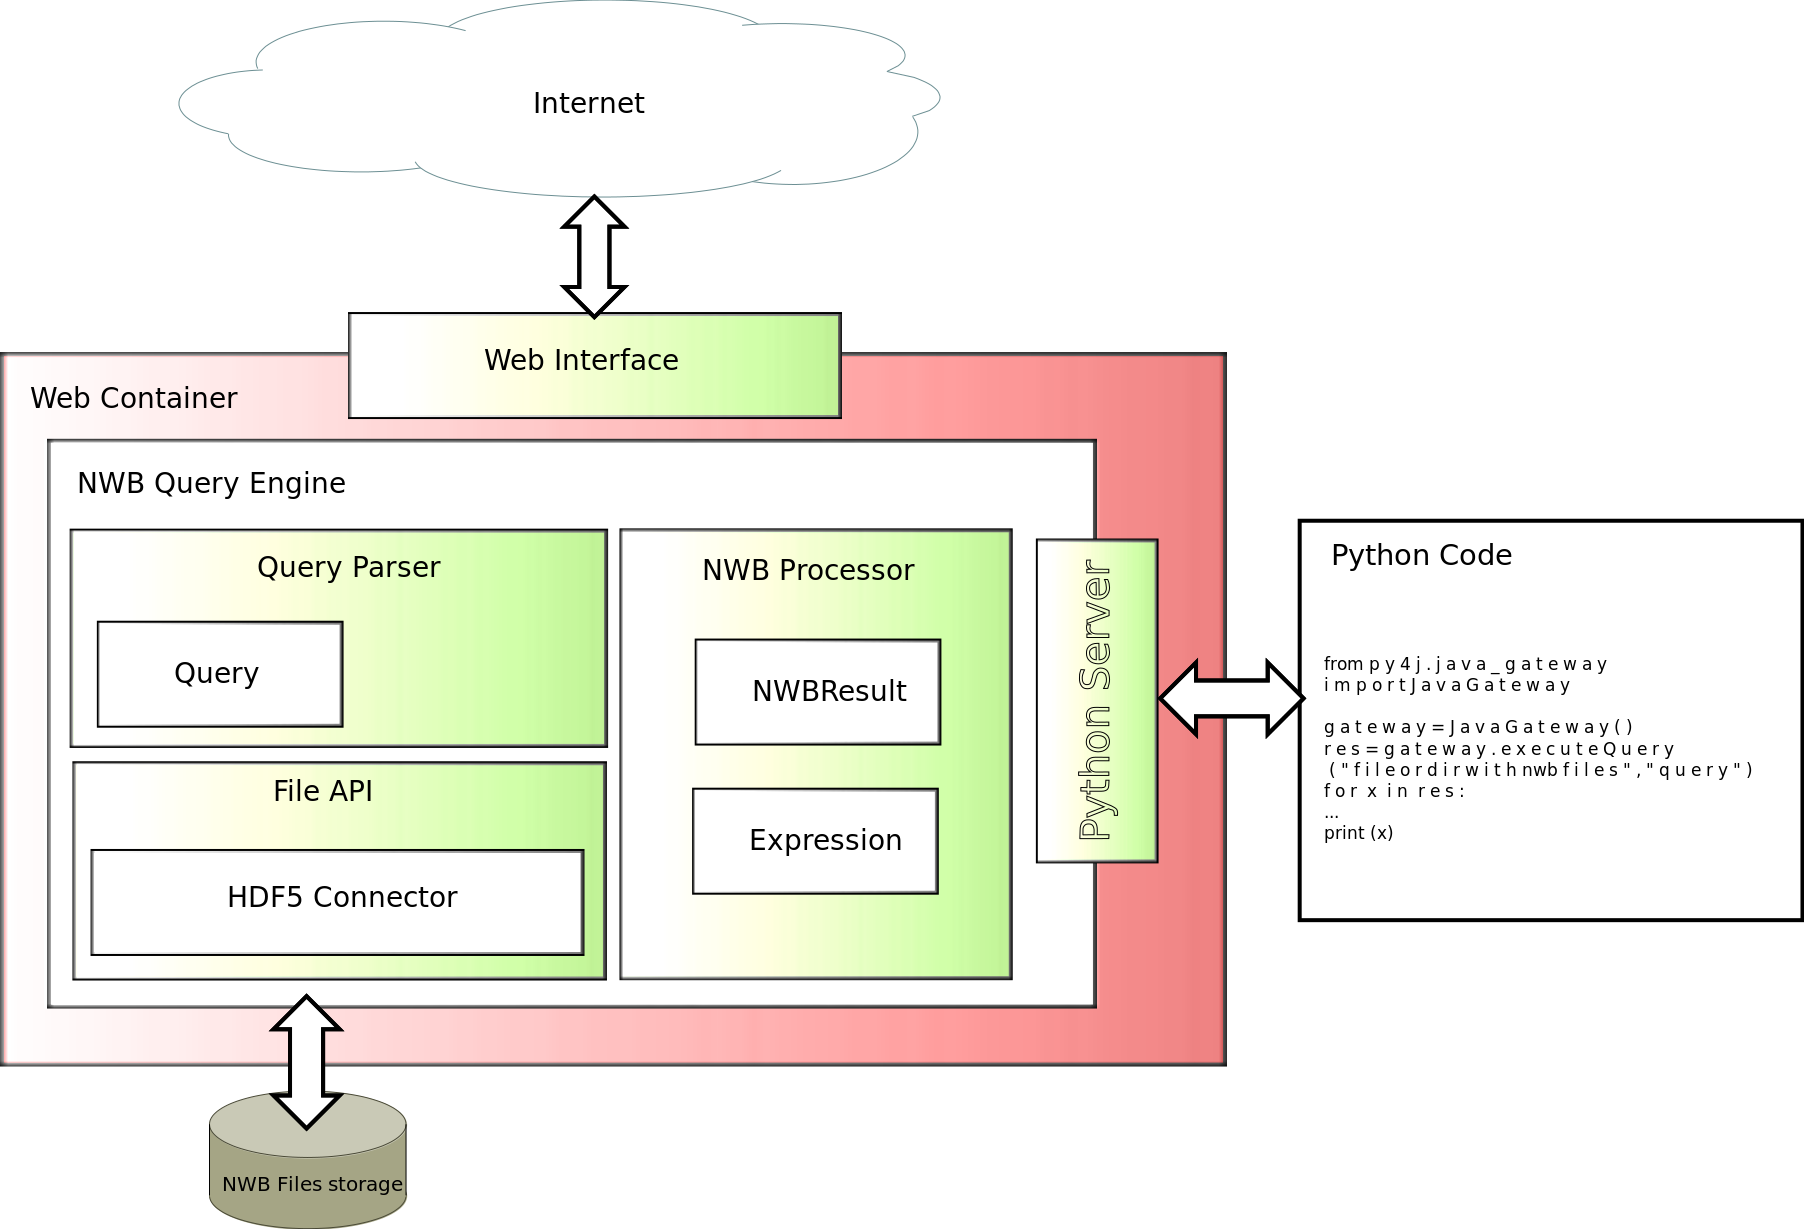
\includegraphics[width=17cm]{architecture}
% figure caption is below the figure
\caption{Block Diagram of the Architecture of the NWB Query Engine}
\label{fig:architecture}
\end{figure}


--connectors interfaces

\subsection{Implementation}
\label{Implementation}

\begin{figure}
% Use the relevant command to insert your figure file.
% For example, with the graphicx package use
  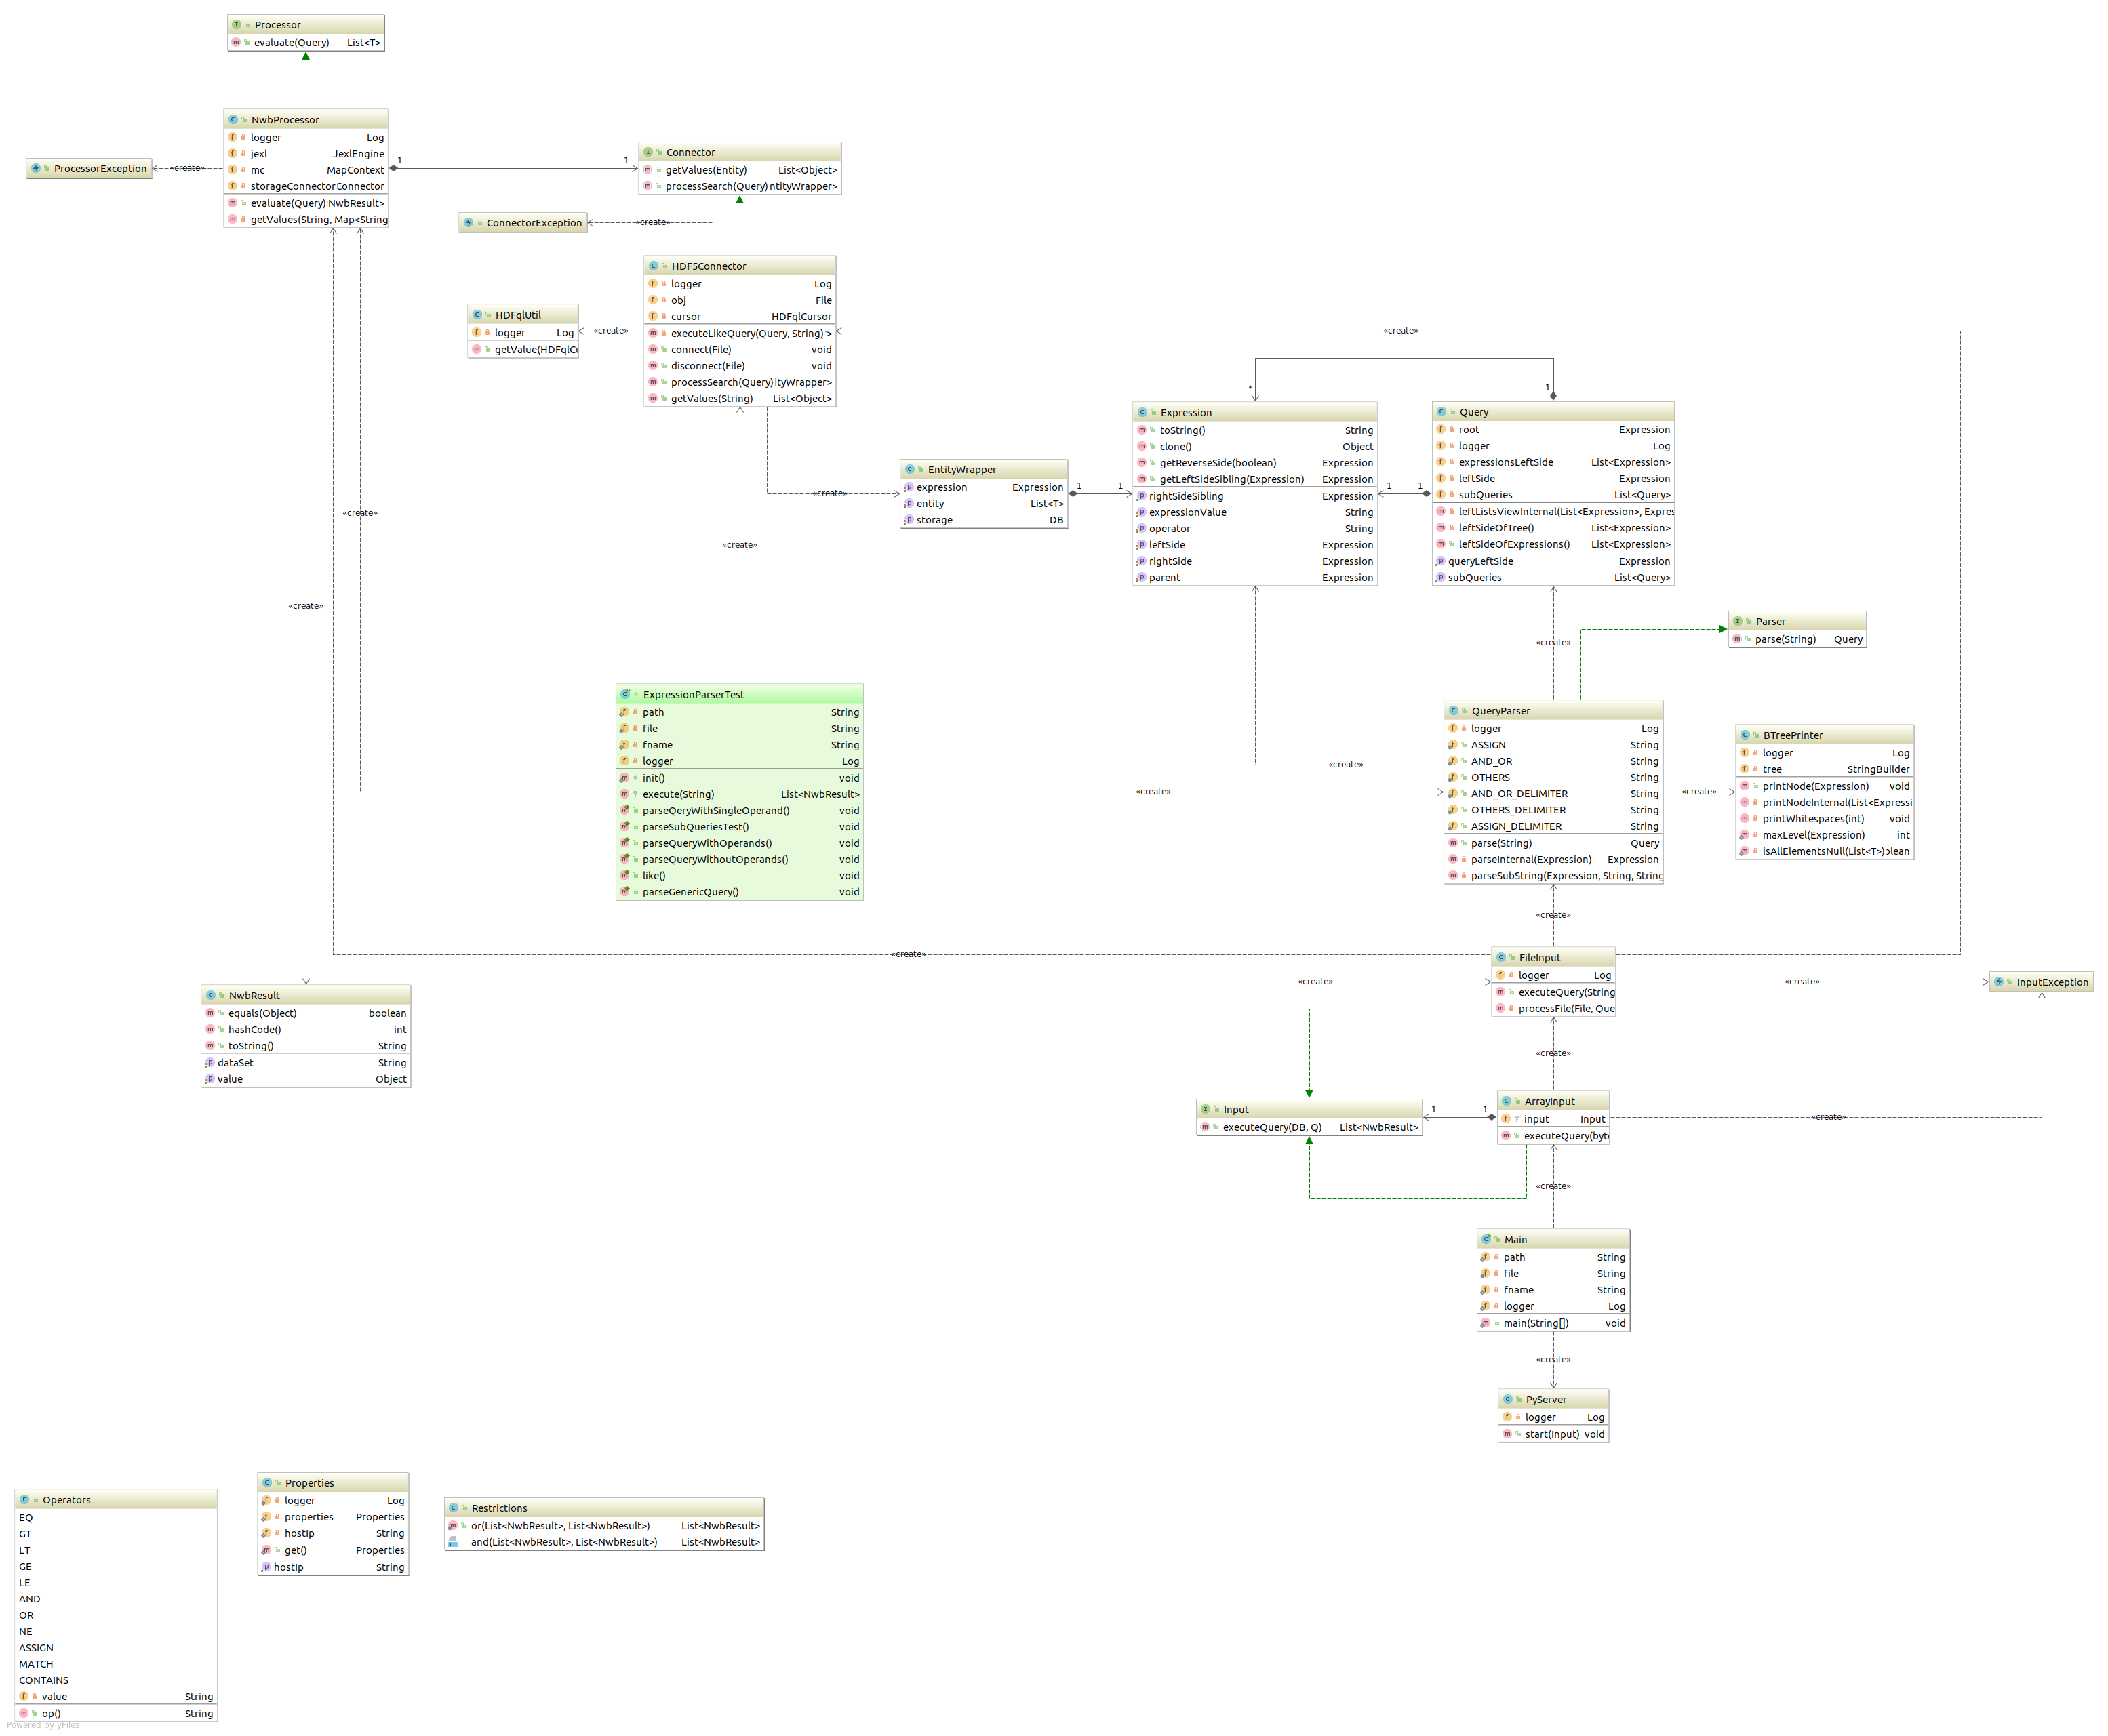
\includegraphics[width=17cm]{diagram}
% figure caption is below the figure
\caption{UML Diagram of the NWB Query Engine}
\label{fig:diagram}
\end{figure}

\subsubsection{Query Grammar}
\label{Query_Grammar}


\begin{tikzpicture}[
    fact/.style={rectangle, draw=none, rounded corners=1mm, fill=blue, drop shadow,
        text centered, anchor=north, text=white},
    state/.style={circle, draw=none, fill=orange, circular drop shadow,
        text centered, anchor=north, text=white},
    leaf/.style={rectangle, draw=none, fill=red, circular drop shadow,
        text centered, anchor=north, text=white},
    level distance=0.5cm, growth parent anchor=south
]
\node (Fact01) [fact] {$epochs=(start\_time>200\&stop\_time<400)$} [->]
        child{ [sibling distance=7cm]
            node (State01) [state] {$=$}
            child{
                node (Fact02) [fact] {$epochs$}
                }
            child{ [sibling distance=4cm]
                node (Fact10) [fact] {$start\_time>200\&stop\_time<400$}
                child{ [sibling distance=8cm]
                    node (State10) [state] {$\&$}
                    child{
                        node (Fact11) [fact] {$start\_time>200$}
                        child{ [sibling distance=2cm]
                            node (State11) [state] {$>$}
                            child{
                              node (Start_Time) [leaf] {$start\_time$}
                            }
                            child {
                              node (200_value) [leaf] {$200$}
                            }
                        }
                    }
                    child{
                        node (Fact12) [fact] {$stop\_time<400$}
                        child{[sibling distance=2cm]
                            node (State12) [state] {$<$}
                            child{
                                node (Fact13) [leaf] {$stop\_time$}
                            }
                            child{
                                node (Fact14) [leaf] {$400$}
                            }
                        }
                    }
                }
            }
        }
;
        
\end{tikzpicture}

\begin{itemize}  
\item gd = group|dataset
\item da = dataset|attribute
\item gd = (expression)
\item expression = expression | expression \& expression
\item expression = da < const | da <= const | da > const | da <= const | da LIKE const | gda
\end{itemize}

% For tables use
\begin{table}
% table caption is above the table
\caption{Query Examples}
\label{tab:query-examples}       % Give a unique label
% For LaTeX tables use

-- include also examples of roots whenever in the hierarchy


\begin{tabular}{ |p{7cm}|p{9cm}| }
\hline
	 \textbf{Query}                                  &       \textbf{Description} \\ \hline
	
	 analysis=(description LIKE whisker)  &  selects all datasets description from an analysis group which contains a whisker string  \\ \hline
	 processing=(electrode\_idx > 30)        &  selects all electrode\_idx datasets from a processing group which value > 30   \\ \hline
	 epochs=(start\_time > 200 \& stop\_time<400 \& stop\_time > 1600)  &  selects all epochs which start\_time > 200 and stop\_time < 400 or stop\_time > 1600 \\ \hline
	 epochs=(start\_time)                     &  selects all epochs with a start\_time dataset         \\ \hline
	 data=(unit LIKE unkno)  &  selects all datasets data with attributes containing a substring unkno \\ \hline
	 pole\_in/data=(unit LIKE unkno)  &  takes into account only data within a pole\_in group \\ \hline
	 analysis=(description LIKE whisker) \& epochs=(start\_time)   &  A combination of previous queries \\ \hline

\end{tabular}

\end{table}



\subsubsection{Operators}


\begin{itemize}
 \item and \&
 \item or  |
 \item equal ==
 \item assignment =
 \item brackets ()
 \item substrings in strings LIKE
\end{itemize}


\subsection{Python Gateway}
\label{Python_Gateway}

\begin{lstlisting}
 >>> from py4j.java_gateway import JavaGateway
 >>> from py4j.java_gateway import GatewayParameters
 >>> gateway = JavaGateway() # for localhost
 >>> gateway = JavaGateway(gateway_parameters=GatewayParameters(address='remote host ip')) # or for remote host
 >>> res = gateway.executeQuery("file or dir with nwb files", "query")
 >>> for x in res:
 ...     print (x)
\end{lstlisting}

\subsection{Web interface}
\label{web_interface}

\begin{figure}
% Use the relevant command to insert your figure file.
% For example, with the graphicx package use
  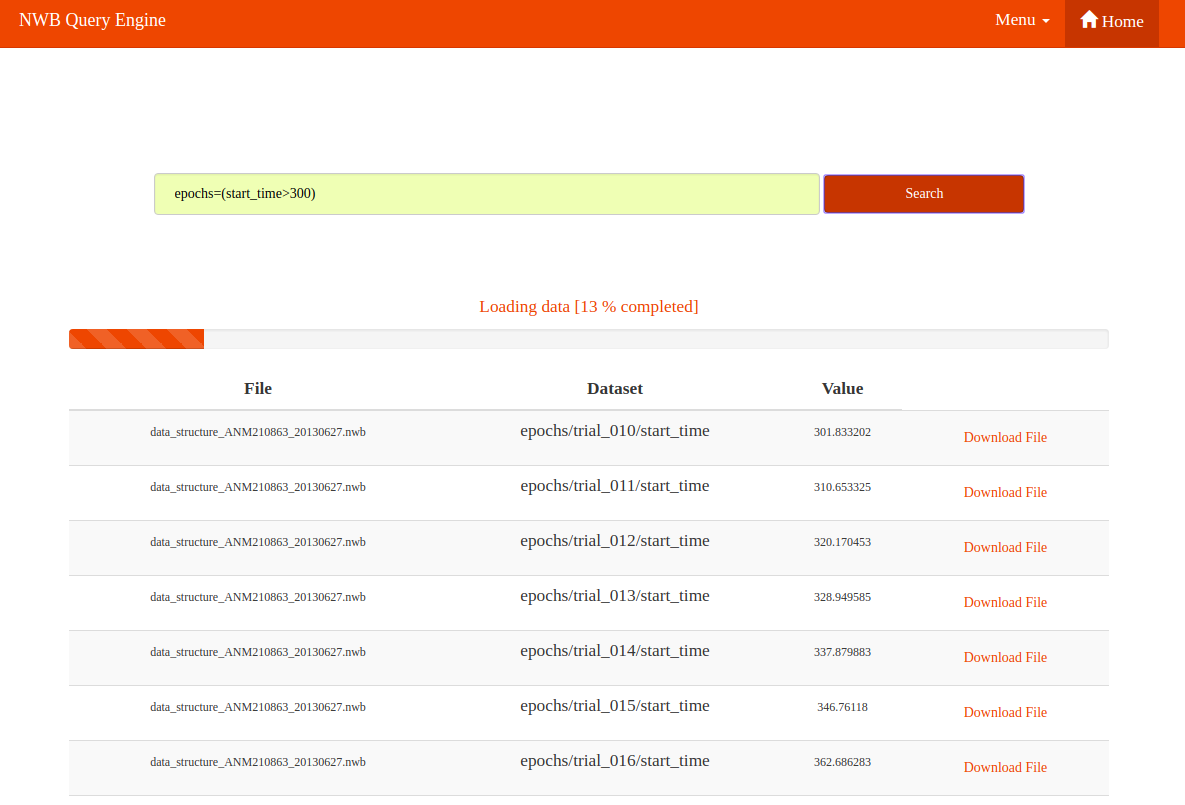
\includegraphics[width=17cm]{nwb-query-engine-web}
% figure caption is below the figure
\caption{NWB Query Engine Web Interface Preview}
\label{fig:diagram}
\end{figure}

\subsection{User Guide}
install steps etc.

Can be run as a library, as a command line application, as a python gateway or from the web

examples?

\section{Discussion}
\label{Discussion}

!todo! Comparrision of DataJoint, limitations of HDFql, why NWB Query Engine is such a good tool. What are its limits, how to solve them in the future?



\section*{Conflict of Interest Statement}
%All financial, commercial or other relationships that might be perceived by the academic community as representing a potential conflict of interest must be disclosed. If no such relationship exists, authors will be asked to confirm the following statement: 

The authors declare that the research was conducted in the absence of any commercial or financial relationships that could be construed as a potential conflict of interest.

\section*{Author Contributions}

The Author Contributions section is mandatory for all articles, including articles by sole authors. If an appropriate statement is not provided on submission, a standard one will be inserted during the production process. The Author Contributions statement must describe the contributions of individual authors referred to by their initials and, in doing so, all authors agree to be accountable for the content of the work. Please see  \href{http://home.frontiersin.org/about/author-guidelines#AuthorandContributors}{here} for full authorship criteria.

\section*{Funding}
Details of all funding sources should be provided, including grant numbers if applicable. Please ensure to add all necessary funding information, as after publication this is no longer possible.

\section*{Acknowledgments}
This is a short text to acknowledge the contributions of specific colleagues, institutions, or agencies that aided the efforts of the authors.

\section*{Supplemental Data}
 \href{http://home.frontiersin.org/about/author-guidelines#SupplementaryMaterial}{Supplementary Material} should be uploaded separately on submission, if there are Supplementary Figures, please include the caption in the same file as the figure. LaTeX Supplementary Material templates can be found in the Frontiers LaTeX folder 


\bibliographystyle{frontiersinSCNS_ENG_HUMS} % for Science, Engineering and Humanities and Social Sciences articles, for Humanities and Social Sciences articles please include page numbers in the in-text citations
%\bibliographystyle{frontiersinHLTH&FPHY} % for Health, Physics and Mathematics articles
\bibliography{nwb-query-engine}

%%% Make sure to upload the bib file along with the tex file and PDF
%%% Please see the test.bib file for some examples of references


\end{document}
